% !TEX root = Anhang.tex

\anhangstart

\phantomsection		
\addstarredchapter{\textbf{Anhang 1, Fragebogen}} % F�gt "Glossar" zum Inhaltsverzeichnis hinzu	
\chapter*{Anhang 1, Fragebogen}

% Abbildung
\begin{figure}[H]
	\centering
	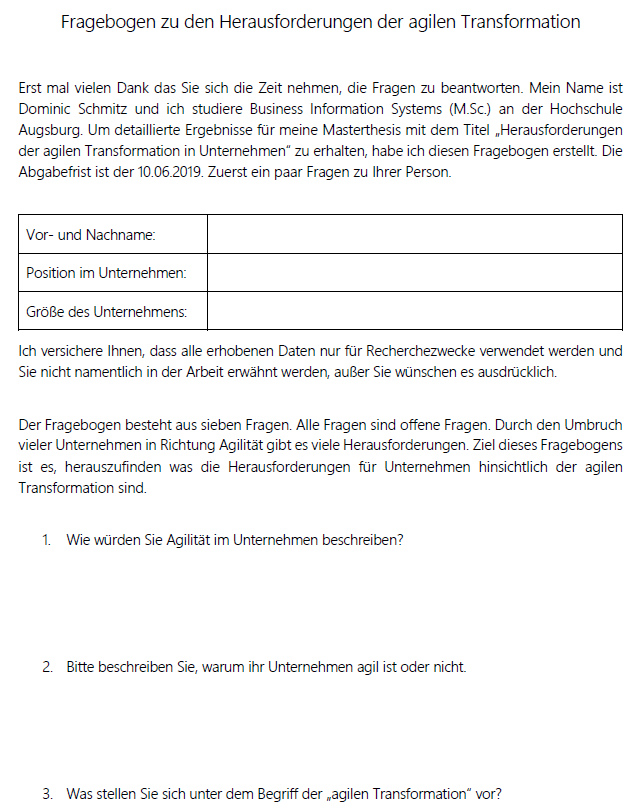
\includegraphics[width=1.0\textwidth]{06_Bilder/Fragebogen_s1.png}
	\setlength{\abovecaptionskip}{1em}
	\caption[]{Fragebogen Seite 1}
	\label{img:anh:fragebogen_s1}
\end{figure}

% Abbildung
\begin{figure}[H]
	\centering
	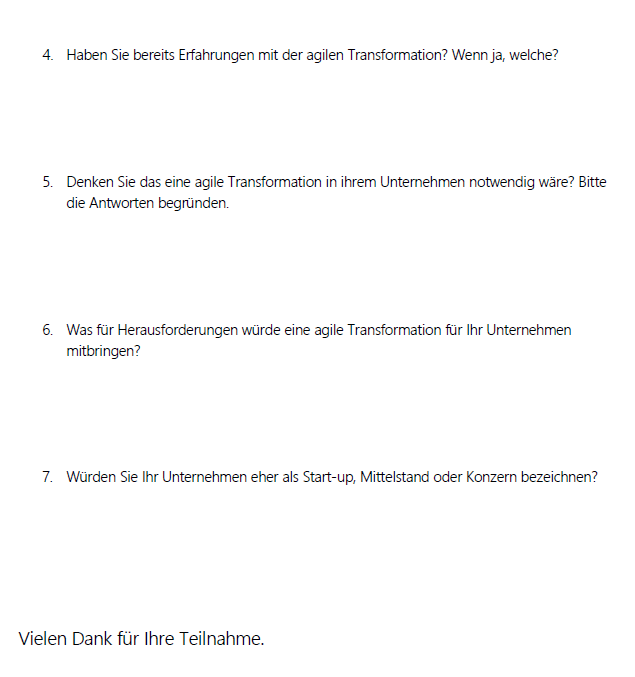
\includegraphics[width=1.0\textwidth]{06_Bilder/Fragebogen_s2.png}
	\setlength{\abovecaptionskip}{1em}
	\caption[]{Fragebogen Seite 2}
	\label{img:anh:fragebogen_s2}
\end{figure}
